% ----------------------------------------------------------
% Subseção Consciência
% ----------------------------------------------------------
\subsection{Consciência}
Como visto na seção do teorema central do limite, um momento lógico é formado por divisão e subdivisões lógicas, como são as subunidades de espaço ou tempo. Um momento lógico (cada linha da Figura \ref{fig:consciousness_logical_moments}) é a soma de suas subunidades lógicas, ou seja, uma unidade.

\begin{figure}[H]
\caption{Intervalo lógico}
\label{fig:consciousness_logical_moments}
\centering
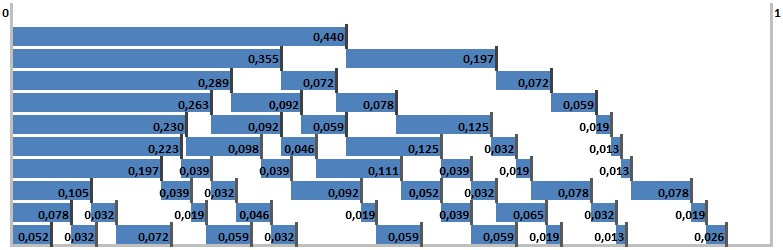
\includegraphics[scale=.7]{sections/images/consciousness_logical_moments.jpg}
\floatfoot{Exemplo de um intervalo lógico com dez momentos lógicos.}%\footnotemark}
\end{figure}
%\footnotetext{Fonte: note}

A consciência são os momentos lógicos de um intervalo representados em suas unidades.

\begin{figure}[H]
\caption{Intervalo lógico consciente}
\label{fig:consciousness}
\centering
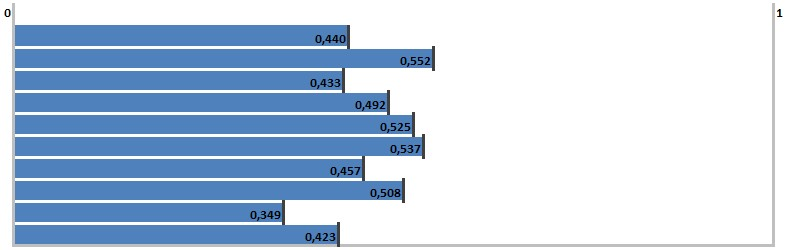
\includegraphics[scale=.7]{sections/images/consciousness.jpg}
\floatfoot{Exemplo de um intervalo lógico consciente com dez unidades de momentos lógicos.}%\footnotemark}
\end{figure}
%\footnotetext{Fonte: note}

Pode ser observado na Tabela \ref{tab:10000_all} que a probabilidade de 99,99\% das amostras, que aumentam em quantidade a medida que crescem os momentos lógicos, tendem a estar cada vez mais ao centro do intervalo lógico, sendo que essa centralização tende ao infinito.

\begin{figure}[H]
\caption{Centralização de 99,99\% das amostras}
\label{fig:centering_of_99_range}
\centering
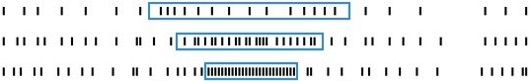
\includegraphics[scale=1]{sections/images/centering_of_99_range.jpg}
\floatfoot{Tendência de centralização do range de 99,99\% das amostras.}%\footnotemark}
\end{figure}
%\footnotetext{Fonte: note}

A consciência é o conjunto dos momentos lógicos de um intervalo. É o aspecto da lógica que unifica as amostras desses momentos, ou seja, é a lógica que abstrai muitos em um, muitas subunidades em uma unidade por momento lógico. Todos os aspectos listados abaixo são inerentes a abstração da lógica chamada consciência.

\subsubsection{Infinito}
Um dos aspectos mais importantes que a negação do nada traz (negação de si), é o infinito, ou seja, em qualquer intervalo lógico cabe o infinito novamente. A lógica primordial que iniciou todo o intervalo lógico é a mesma encontrada em seus intervalos subsequentes. Não há fim, não há meio, apenas infinitos começos. Isso fundamenta como uma lógica de alto nível como a consciência explica a lógica primordial, uma vez que não é preciso voltar ao primeiro momento lógico do intervalo para deduzi-lo, pois esse fenômeno é onipresente em todo o intervalo.

\subsubsection{Ondas e subconsciente}
Probabilisticamente a distribuição de novas amostras de uma população tendem a concentrar mais amostras sentido a mediana da população com frequências de amostras cada vez maiores neste sentido. Porém, a distribuição dessas amostras com frequências de crescimento uniformes é infinitesimal se comparado às possibilidades randômicas desse crescimento. Assim, a tendência de crescimento dessas frequências sentido a mediana somadas a baixíssima probabilidade (infinitesimal) desse crescimento ser uniforme, conduz a frequências no padrão de ondas.

\begin{figure}[H]
\caption{Padrão de onda}
\label{fig:consciousness_waves}
\centering
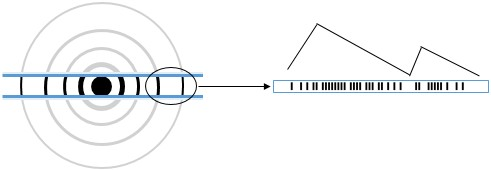
\includegraphics[scale=1]{sections/images/consciousness_waves.jpg}
\floatfoot{Padrão de onda inferido pela tendência dessa distribuição com frequências maiores sentido a mediana da população e a baixíssima probabilidade de crescimento uniforme dessas frequências.}%\footnotemark}
\end{figure}
%\footnotetext{Fonte: note}

As amostras que mais se parecem em termos de frequências e distribuição são as amostras que fazem parte da mesma onda, que em momentos passados estiveram mais próximas. Elas são frequências opostas não sobrepostas que se completam. Essas ondas formas subconsciência de uma consciência maior. A consciência é única para todo o intervalo, é a lógica do intervalo, enquanto forma subconsciências, como pequenas ondas de uma onda maior. Assim, uma mudança na onda maior (consciência) também é uma mudança na onda menor (subconsciência), mudança essa que é induzida pela subconsciência indiretamente, análogo ao comprimir gás em um cilindro, ao adicionar uma nova molécula de gás no cilindro parcialmente cheio mais próximas ou apertas essas moléculas dentro dele estarão. O contrário também é verdadeiro, uma nova amostra em uma subconsciência, que por esta é observada diretamente é também uma mudança da consciência e vai ser induzida pelas outras subconsciências indiretamente.

\begin{figure}[H]
\caption{Subconsciência}
\label{fig:consciousness_subconscious}
\centering
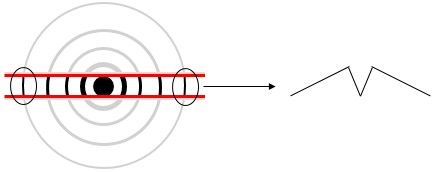
\includegraphics[scale=1]{sections/images/consciousness_subconscious.jpg}
\floatfoot{O padrão de ondas forma subconsciências semelhantes ao padrão criado pela consciência como visto na Figura \ref{fig:statisticsbyjim_central_limit_theorem} ou na Figura \ref{fig:trend_chart_of_normal_distribution}.}%\footnotemark}
\end{figure}
%\footnotetext{Fonte: note}

Grandes intervalos com baixas frequências de amostras ou grandes intervalos com frequências uniformes de amostras são mais difíceis de observar devido à ausência de grandes discrepâncias. A junção de duas ondas além de eliminar suas discrepâncias, faz com que a primeira onda da união fique maior e a segunda onda acaba por deixar de existir e se tornar parte da primeira que tem seu pico mais próximo da mediana. Probabilisticamente uma onda não morre, apenas une-se com outras ondas mais internas a ela.

\begin{figure}[H]
\caption{Unificação de ondas}
\label{fig:consciousness_uniform_wave}
\centering
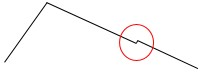
\includegraphics[scale=1]{sections/images/consciousness_uniform_wave.jpg}
\floatfoot{Ondas sendo unificadas para exemplificar o crescimento amostral uniforme.}%\footnotemark}
\end{figure}
%\footnotetext{Fonte: note}

Probabilisticamente as duas partes complementares de uma onda estarão a uma distância aproximadamente iguais, equidistante da mediana, porém essa não é uma regra e isso abre caminho para o entrelaçamento quântico, onde as partes complementares de uma onda podem estar em distancias diferentes da mediana. 

\subsubsection{Espaço}
As ondas da consciência exibidas em forma de histograma, onde as partes da onda que se completam são colocados lado a lodoé exibida na Figura \ref{fig:consciousness_space_waves}. 
\begin{figure}[H]
\caption{Histograma em padrão de ondas}
\label{fig:consciousness_space_waves}
\centering
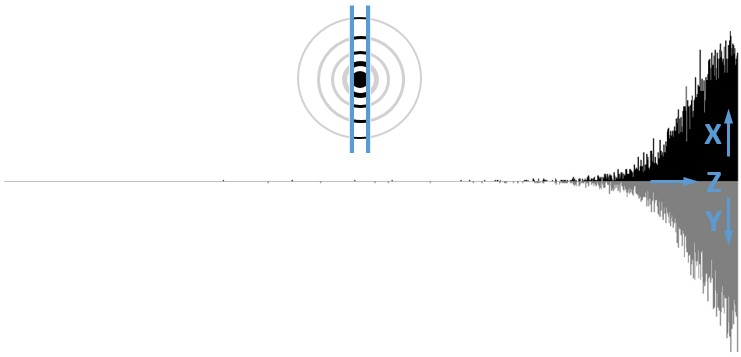
\includegraphics[scale=.7]{sections/images/consciousness_space_waves.jpg}
\floatfoot{Exemplo de padrão de ondas obtido pelo algoritmo Logic\_WavePattern \footnotemark.}
\end{figure}
\footnotetext{O algoritmo Logic\_WavePattern pode ser visto no Apêndice \ref{app:algoritmos}.}

Ao representar as grandezas espaciais conforme o gráfico a Figura \ref{fig:consciousness_space_waves} e distribuir seus pontos de extremidade em um gráfico de distribuição 3D, obtém-se algo parecido com uma espiral mesmo em volume muito pequeno de dados, conforme \ref{fig:consciousness_space_3DScatter}. 
\begin{figure}[H]
\caption{Gráfico de dispersão 3D gerado com os pontos do histograma em padrão de ondas}
\label{fig:consciousness_space_3DScatter}
\centering
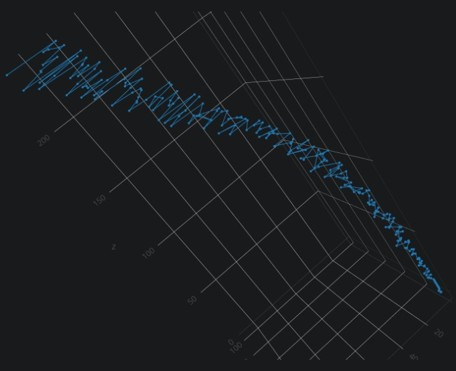
\includegraphics[scale=1]{sections/images/consciousness_space_3DScatter.jpg}
\floatfoot{O histograma no padrão de ondas e os dados para gerar o gráfico de dispersão 3D podem ser obtidos com a execução do algoritimo Logic\_WavePattern \footnotemark.}
\end{figure}
\footnotetext{O algoritmo Logic\_WavePattern pode ser visto no Apêndice \ref{app:algoritmos} e o gráfico de dispersão 3D pode ser acessado em: \url{https://chart-studio.plot.ly/create/?fid=ren.stuchi:5&fid=ren.stuchi:4}}

Observações que podem ser feitas com a Figura \ref{fig:consciousness_space_subconsciousness}:
\begin{itemize}
  \item Quanto mais próximas da mediana mais largas (dimensão Z), mais altas (dimensões X e Y) as subconsciências se tornam.
  \item Quanto mais próximos da mediana mais subconsciências aninhadas se formam, representadas por cores diferentes. 
  \item As primeiras subconsciências (azul claro) tendem a ter seus volumes muito mais expressivo que os volumes das demais. Já as últimas subconsciências tendem ser muito finas e compridas. Pode ser comparado com as galáxias com seus núcleos extremamente volumosos (azul claro), depois as estrelas com enormes volumes, passando pelos planetas (subconsciências aninhadas bem menores) até os átomos ou estruturas menores que são muito pequenas, se apresentam em enormes quantidades e as partículas que orbitam seu núcleo ficam bem mais distantes dele.
  \item Provavelmente, o padrão aproximado de espiral visto na Figura \ref{fig:consciousness_space_3DScatter} das primeiras consciências (azul claro) também refletirão nas subconsciências posteriores, pois estas são partes da primeira e assim por diante.
\end{itemize}
\begin{figure}[H]
\caption{Abstração espacial das subconsciências}
\label{fig:consciousness_space_subconsciousness}
\centering
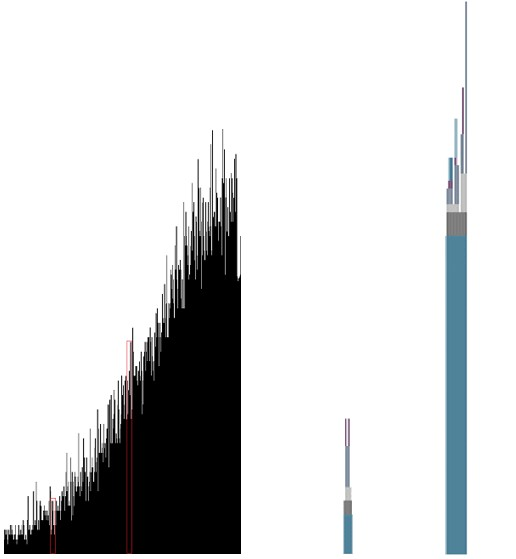
\includegraphics[scale=.8]{sections/images/consciousness_space_subconsciousness.jpg}
\floatfoot{Caracteristicas da ondas formadoras da subconsciência.}%\footnotemark}
\end{figure}
%\footnotetext{Fonte: note}

A observação das subconsciências depende do range de ondas que elas conseguem observar e esse range, por sua vez depende do range de ondas que a própria subconsciência é constituída. Em partículas muito pequenas como os elétrons pode-se notar o salto quântico \cite{universoracionalista_salto_quanticos}. Alguns equipamentos (sub-lógicas) podem melhorar essas observações, se aprofundar em detalhes, ou seja, visualizar blocos de amostras ainda menores e menores até que se possa visualizar uma única amostra.  
\begin{figure}[H]
\caption{Observações subconscientes}
\label{fig:consciousness_space_subconscious_observation}
\centering
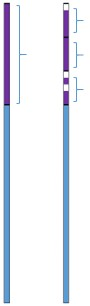
\includegraphics[scale=.9]{sections/images/consciousness_space_subconscious_observation.jpg}
\floatfoot{Diferentes subconsciências diferentes observações dos intervalos de ondas.}%\footnotemark}
\end{figure}
%\footnotetext{Fonte: note}


\subsubsection{Tempo}
O tempo é a adição de novos momento lógicos à medida que prossegue a negação desses momentos.  Essas mudanças são acumulativas e a medida que aumentam os número de amostras ou momentos lógicos, menos relevante cada nova amostra será dentro do intervalo consciente. Um em cem é mais relevante do que um em mil. 

\begin{figure}[H]
\caption{Tempo}
\label{fig:consciousness_time}
\centering
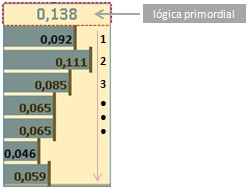
\includegraphics[scale=.8]{sections/images/consciousness_time.jpg}
\floatfoot{Progressão do tempo conforme os momentos lógicos avançam.}%\footnotemark}
\end{figure}
%\footnotetext{Fonte: note}

Outro fator importa a observar do tempo é que, probabilisticamente, subconsciências mais próximas da mediana da população terão uma adição maior de novas amostras em seus intervalos, o que são observados diretamente por essas subconsciências. Por outro lado, subconsciências distantes da mediana da população terão uma adição menor de amostras em seus intervalos e sujeitam-se a um número maior de mudança induzidas pela subconsciência indiretamente. Esse fenômeno de observação temporal proporcionado pela consciência e subconsciências evita o paradoxo dos gêmeos \cite{brasilescola_paradoxo_gemeos}.

Na seção Expansão binomial foi apresentado que a lógica é uma sequência de negações de si no tempo zero, ou seja, em nenhum momento entre suas negações a lógica passa a SER, garantindo a premissa primordial da constante lógica NÃO SER. Assim, a lógica é uma sequência infinita e simultânea, uma constante.
Logo, o tempo é apenas uma grandeza da consciência oriunda da sequência lógica. A simultaneidade dessa sequência torna a lógica uma constante com todas as suas infinitas possibilidades, sendo esse universo uma delas. Cada universo tem sua sequência de mudanças, que é estática, em uma ordem diferente e é essa ordem que dá origem à grandeza que chamamos de tempo. É essa ordem do universo ou consciência que vai dar a noção do que acontece antes ou depois, ou seja, o passado, o presente e o futuro.
Na experiência do tempo conduzida pela consciência a ordenação da sequência é a essência dessa grandeza e, portanto, mais relevante do que sua origem que é de natureza simultânea.


\subsubsection{Gravidade}
A gravidade é um aspecto probabilístico da distribuição amostral de uma população, como previsto pelo teorema central do limite. Esse teorema afirma que a distribuição amostral de uma população se aproxima de uma distribuição normal à medida que o tamanho das amostras aumentam, o que tende probabilisticamente à centralização infinita das amostras conforme os momentos lógicos progridem. A atração do amor, a gravidade que atraem os objetos à terra e a terra ao sol são sinônimos deste mesmo aspecto. Em outras palavras, a gravidade é análoga a uma conexão que fica cada vez mais forte a medida que se aproxima da mediana, onde tem-se uma concentração de amostras cada vez maior.

\begin{figure}[H]
\caption{Gravidade}
\label{fig:consciousness_gravity}
\centering
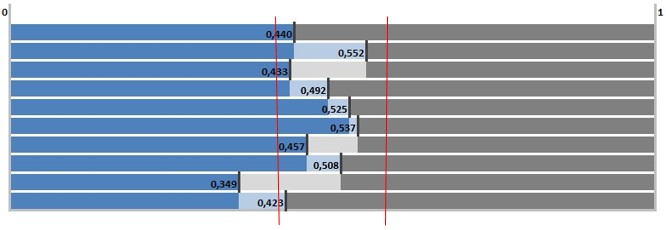
\includegraphics[scale=.8]{sections/images/consciousness_gravity.jpg}
\floatfoot{Centralização infinita das amostras conforme os momentos lógicos progridem.}%\footnotemark}
\end{figure}
%\footnotetext{Fonte: note}

\subsubsection{Matéria escura e energia escura}
Quanto maior o número de amostras e mais próximas elas estão da mediana, mais elas farão parte dos 99,99\% e ainda mais amostras também estarão nos 0,01\%, conforme a Tabela \ref{tab:10000_all}. Assim, a observação desses 0,01\% passa a ser cada vez mais difícil, pois sua relevância consciente passa a ser cada vez mais próxima de zero. É importante notar também que a medida que os 99,99\% aumentam em número de amostras, menos relevante cada nova amostra será dentro desse conjunto (um em cem é mais relevante do que um em mil) e uma porcentagem menor será ocupada pelo range dos 99,99\% das amostras, conforme a Tabela \ref{tab:10000_all}.

\begin{figure}[H]
\caption{Analogia da matéria escura e energia escura}
\label{fig:consciousness_dark_matter_dark_energy}
\centering
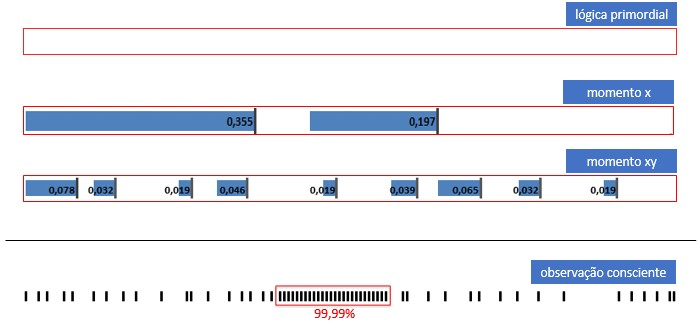
\includegraphics[scale=1]{sections/images/consciousness_dark_matter_dark_energy.jpg}
\floatfoot{Fenômenos antevistos ou conjecturados pela consciência.}%\footnotemark}
\end{figure}
%\footnotetext{Fonte: note}

\subsubsection{Antimatéria}
Independente do intervalo observado (análogo à bytes, kilobytes, prótons, elétrons etc.), que são contextos lógicos de observação e/ou utilização consciente, este pode estar com sua maior concentração de amostras no sentido da mediana, o que é o sentido provável conforme os números de amostras crescem em um intervalo, conforme teorema central do limite. Essas amostras também podem estar com sua concentração no sentido oposto a mediana, porém com uma ocorrência probabilística cada vez menos conforme as amostras aumentam. Na Figura \ref{fig:consciousness_concentration_of_opposite_samples} é exibido dois intervalos idênticos com suas amostras com concentrações opostas.

\begin{figure}[H]
\caption{Parte de um intervalo idêntico com suas concentrações de amostras opostas}
\label{fig:consciousness_concentration_of_opposite_samples}
\centering
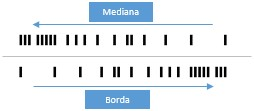
\includegraphics[scale=1]{sections/images/consciousness_concentration_of_opposite_samples.jpg}
\floatfoot{Parte de um intervalo idêntico distribuídos de formas opostas.}%\footnotemark}
\end{figure}
%\footnotetext{Fonte: note}

O merge ou soma dos intervalos opostos da Figura \ref{fig:consciousness_concentration_of_opposite_samples} os tornaria um intervalo simétrico, ou seja, não estaria em nenhum dos sentidos.
Na Figura \ref{fig:consciousness_concentration_of_opposite_samples_within_range} é exibido um intervalo consciente completo com suas concentrações de amostras sentido à mediana e outro idêntico, mas com suas concentrações sentido às bordas do intervalo.

\begin{figure}[H]
\caption{Intervalos conscientes com suas concentrações de amostras opostas}
\label{fig:consciousness_concentration_of_opposite_samples_within_range}
\centering
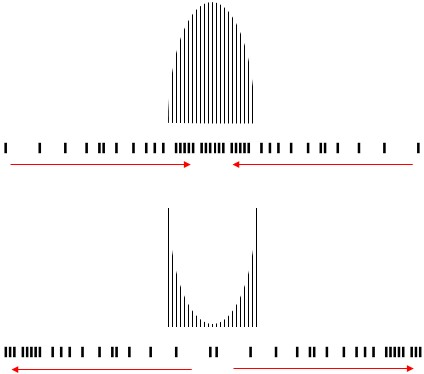
\includegraphics[scale=.8]{sections/images/consciousness_concentration_of_opposite_samples_within_range.jpg}
\floatfoot{Intervalos conscientes completos e idênticos distribuídos de formas opostas.}%\footnotemark}
\end{figure}
%\footnotetext{Fonte: note}


\subsubsection{Buraco negro}
O buraco negro é uma concentração muito alta de amostras, uma altíssima frequência de amostras em um intervalo lógico, que muito provavelmente, em um passado distante dessa consciência esteve muito próximo ao centro dessa consciência, é o pico de uma onda, onde devido ao alto número não há mais discrepância, ou seja, é um pico de onda com um crescimento uniforme e por isso inobservável. 

\begin{figure}[H]
\caption{Buraco negro}
\label{fig:consciousness_black_hole}
\centering
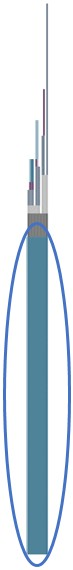
\includegraphics[scale=1]{sections/images/consciousness_black_hole.jpg}
\floatfoot{Centralização infinita das amostras em uma proporção centralizada cada vez menor.}%\footnotemark}
\end{figure}
%\footnotetext{Fonte: note}